% ****** Start of file aipsamp.tex ******
%
%   This file is part of the AIP files in the AIP distribution for REVTeX 4.
%   Version 4.1 of REVTeX, October 2009
%
%   Copyright (c) 2009 American Institute of Physics.
%
%   See the AIP README file for restrictions and more information.
%
% TeX'ing this file requires that you have AMS-LaTeX 2.0 installed
% as well as the rest of the prerequisites for REVTeX 4.1
%
% It also requires running BibTeX. The commands are as follows:
%
%  1)  latex  aipsamp
%  2)  bibtex aipsamp
%  3)  latex  aipsamp
%  4)  latex  aipsamp
%
% Use this file as a source of example code for your aip document.
% Use the file aiptemplate.tex as a template for your document.
\documentclass[%
 aip,
 jmp,%
 amsmath,amssymb,
%preprint,%
 reprint,%
%author-year,%
%author-numerical,%
]{revtex4-1}


\usepackage{graphicx}% Include figure files
\usepackage{dcolumn}% Align table columns on decimal point
\usepackage{bm}% bold math
%\usepackage[mathlines]{lineno}% Enable numbering of text and display math
%\linenumbers\relax % Commence numbering lines

\usepackage{algorithm}
\usepackage[noend]{algpseudocode}

\begin{document}

\preprint{AIP/123-QED}

\title[]{Confinement Induced Electron Capture}

\author{C. Martin}
 \altaffiliation[Also at ]{Physics Department, XYZ University.}%Lines break automatically or can be forced with \\
\author{R. Godes}%
 \email{Second.Author@institution.edu.}
\affiliation{ 
Authors' institution and/or address%\\This line break forced with \textbackslash\textbackslash
}%


\date{\today}% It is always \today, today,
             %  but any date may be explicitly specified

\begin{abstract}
We describe a Gedankenexperiment in which a bare proton can capture an electron due solely to confinement. We first briefly review orbital electron capture and related processes.  We then describe the Fermi VA theory and how it can be applied to compute the cross section and rate using the full relativisitic Kinematics.  We set the problem up as a (proton, electron) pair confined in classical box of size L, and compute the cross section using the full Weak Interaction Hamiltonian.  We provide numerical solutions for electron capture rate, and compare the power output relative to that of a neutron being captured in the post-reaction.  We find that the capture is most likely for L=0.004-0.009 Angstroms, well beyond the radius of the proton and the Compton wavelength of the electron.  We estimate the theoretical minimal power output for such a process, seeing that is feasible at large box lengths.  Finally, we discuss proposals for future work and possible applications.
%
\end{abstract}

\pacs{Valid PACS appear here}% PACS, the Physics and Astronomy
                             % Classification Scheme.
\keywords{Suggested keywords}%Use showkeys class option if keyword
                              %display desired
\maketitle

\section{Background}

As a student, we learn that the nucleus can not contain an electron; this is a simple application of the Heisenberg Uncertainty Principle \cite{Weisskopf}.  If an electron were confined to the volume of a nuclear radius, it would have a (relativisitic) kinetic energy of order $10\;MeV$.  But this is not observed experimentally.  In Beta ($\beta^{-}$) decay, a nucleus emits an electron with energy of order $1\;MeV$: 

$$\beta^{-}\;decay:\;n^{0}\rightarrow p^{+}+\;e^{-}\;+\;\bar{\nu_{e}}$$

We can describe Beta decay using the Fermi VA theory for the Weak Interaction, which assumes a phenomenological contact force \emph{with no range}.

A related Weak process is orbital electron capture, where a nucleus captures a bound, low lying electron, and emits a neutron and an electron anti-neutrino.

$$Electron\;capture:\;p^{+}+\;e^{-}\rightarrow\;n^{0}\;+\;\nu^{e}$$

Orbital electron capture (E.C.) is a fundamental  nuclear process, on pair with the more familiar Beta decay and positron production. It is, however, usually treated as an afterthought to Beta decay, and there are no modern reviews of how to treat the the problem numerically.  Indeed, the most complete reference date back to the 1960s and 70s \cite{ec-review1,ec-review2}.  Still, electron capture displays its own unique, rich structure and subtlety.  For example, the rate is effected chemical environment by nearly $1\%$.    This is because the rate depends on the electronic density on the surface of the nucleus (i.e. $\vert\Psi_{e}(r\rightarrow 0)\vert^{2}$) since the interaction has no range. 

But if we apply the Heisenberg Uncertainty Principle for electron capture, we would find the electron can still be captured even if it is confined to a volume $100X$ the nuclear radius.  

E.C. can also emit Bremsstrahlung radiation.  This is actually discussed in Jackson with a classical model \cite{jackson}, although it is more properly treated using QED corrections to the Weak Interaction\cite{Jauch}.  Technically, electron capture is a 2-body, relativistic bound state problem, although we model it by computing the non-relativistic atomic electronic wavefunctions of the parent and daughter nuclei, and then use them to evaluate the matrix elements of the Weak Interaction Hamiltonian using the Fermi-VA theory.  And very rarely is there a complete treatment of the relativistic Kinematics.


We are interested in the reviewing the basic  electron capture process to   understand how to apply the Fermi-VA theory to compute the cross section and capture rate as completely as possible.  We will examine electron capture in its simplest form:  a bare proton capturing an electron while confined in a classical box.   We don't believe this has been discussed elsewhere and would serve as a basis for more extensive calculations.  

We begin by briefly reviewing both orbital electron capture and, then, the Fermi VA Theory.

\subsection{Orbital Electron Capture}
In 1935, Yukawa proposed that a proton, bound in an atomic nucleus,  could capture a low lying, bound atomic electron, transforming into a neutron, and releasing an electron neutrino:


$$p^{+}+\;e^{-}\rightarrow\;n^{0}\;+\;\nu^{e}$$

This may be called orbital electron capture, K-electron capture, or just electron capture (E.C.) 

Note that unlike Beta decay, which is a 1 body decay, and the emitted electron has a wide energy spectrum, E.C. is a 2 body reaction, and the emitted neutron is mono-chromatic.

Electron capture usually occurs in unstable radioisotopes which lack the nuclear binding energy, $Q$, to decay by the more familiar Beta decay processes ($\beta^{-}, \beta^{+}$). The typical $Q$ energies necessary are 

$$Q_{\beta^{+}}\sim2-4{MeV}$$
$$Q_{\beta^{-}}\sim0.5-2(MeV)$$
$$Q_{E.C.}\sim0.2-2.0{MeV}$$

When $Q<1.02{MeV}$, twice the rest mass of an electron $(2m_{e}c^{2})$, a proton rich nucleus must decay by electron capture.

In particular, heavy elements may decay by E.C. and/or $\beta^{+}$ (positron emission) to a lower 'magic number' of stable nuclei, or by $\beta^{-}$ decay to achieve a higher magic number.    E.C. is favored for high Z nuclei, but because of the energetic constraint, very light elements, such as $^{7}Be$, decay by primarily by E.C.    

Note that lacking any binding energy and/or internal nucleon structure, bare proton electron capture is not readily observed, and requires extreme, exotic conditions such as strong confinement.

\subsubsection{Experimental Evidence}

We observe electron capture by observing the resulting transmuted nuclei and/or the radiative relaxation processes.  The captured electron is bound to the atom, and it is usually a K-shell electron, but may be L or higher.  The nucleus may then absorb some energy, become excited, and undergo internal conversion.  During this, another higher lying, bound atomic electron is absorbed, releasing an X-ray or Auger electron [see Figure \ref{fig:ec1}].

\begin{figure}
   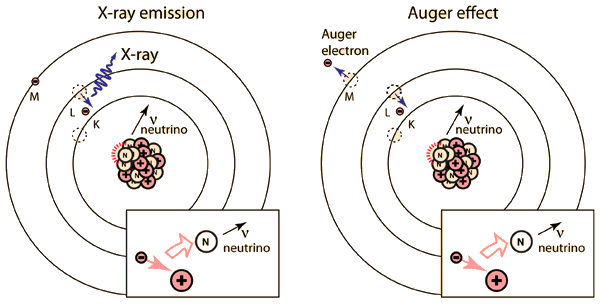
\includegraphics[scale=0.25]{img/ecrelax.png}
   \caption{orbital electron capture relaxation processes}
  \label{fig:ec1}
\end{figure}

Because electron capture occurs in proton-rich nuclei, and, subsequently, releases a X-ray photon, the reaction is also sometimes written as

$$^{Z}X_{A}+\;e^{-}\rightarrow\;^{Z-1}X_{A}\;+\;h\nu_{X-ray}$$

(where A is the total number of protons and neutrons, Z the number protons, and $h\nu_{X-ray}$ is an X-ray photon)

Indeed, orbital electron capture is evidenced by high intensity X-rays and soft electrons.  In 1938, Alvarez observed the X-ray signature of orbital electron capture in activated Titanium \cite{alvarez}. Since then, electron capture has been observed in about 150 radioactive isotopes.


\subsubsection{Environment Effects on Electron Capture rates}

$^{7}Be$ is the  lightest element that E.C. has been observed in \cite{radbook}. In fact, there is so little energy that the competing $\beta^{+}$ positron emission process (described below) is prohibited, leading to a fairly long E.C. half-life of $\tau_{EC}\sim 50\;days$.

Being so light, and having such a large rate, electron capture in $^{7}Be$ can be slightly modified by both changing the chemical environment and/or the external pressure \cite{wang,raydas,ohtsuki}. In particular, in 2004, Ohtsuki et. al. demonstrated a change of $0.83\%$  by embedding Be in C-60 cages \cite{ohtsuki}.

How could such changes occur?  The nuclear energy levels are in the keV to MeV region, and it is generally thought to be very difficult to impossible to effect.  But the electron capture rate is proportional to electronic density at the surface of the nucleus--\emph{the nuclear charge}.   The electronic energy levels are in the eV range, so intense EM fields can alter the electronic structure and therefore slightly affect the E.C. rate. 

\subsubsection{Bare Electron Proton Capture and Stellar Nucleosynthesis}

At zero energy, bare proton electron capture is not possible because it violates energy-momentum conservation. Theoretically, a free proton can could capture an electron from the continuum, but the interaction energy must be above the threshold for neutron production.  This is a huge amount of energy, although this happens regularly in accelerators, and, presumably, in stellar environments.  Observing such capture outside of an accelerator would be an incredibly hard experiment  because both final particles are neutral, and the neutrino is extremely weakly interacting.  

Bare capture is thought to occur in stellar nucleosynthesis because the environment is very dense, and the system is in thermal equilibrium.  This drives the formation of primordial elements, and occur when neutron stars form.    At very high temperatures, the proton electron collisions have sufficient energy to overcome the reaction barrier.   For example, Bachall and coworkers have computed the electron capture rate of $^{7}Be$ in the Sun \cite{bachall62,bachall69}. And it is believed that ionized Hydrogen captures an electron during the core collapse supernovae and in neutron stars [14].   

While we usually characterize a star by it's temperature, these are also very dense systems, with $\rho\sim 10^6\;g\;cm^{-3}$.  In contrast, the smallest star has density $\rho\sim 10^{2}-10^{3}\;g\;cm^{-3}$ [?]  As important, the reverse reaction is prohibited because, inside the dense neutron star, it is impossible to create a new electron; the Fermi sea is \emph{full}.


So electron capture can occur by bare protons, but, presumably, only under extreme confinement, and with the reverse reaction is suppressed.   And there are many studies of numerical rate calculation in high thermal, stellar environments.  We have found none for the kind of confined process we are describing.
We model this numerically particle-in-a-box using the fhe Femi VA theory.

\subsection{The Weak Interaction and Femi VA theory}

Electron capture is mediated by the Weak Interaction, described most concisely by the Fermi VA (Vector Axial) theory. \cite{fermi1,ec-review1,ec-review2}
The VA theory is a simple phenomenological approach, readily amenable to numerical calculations. It is now understood in terms of ElectroWeak Unification and can be derived from the Standard Model.  

The original paper by Fermi, for which he won the 1938 Nobel Prize in Physics, was initially rejected by \emph{Nature} because 

\emph{It contained speculations too remote from reality to be of interest to the reader}.\cite{close}

VA theory can be used to compute cross sections for scattering experiments and decay rates for electron capture for various atoms,  even in different environments, chemical and otherwise.  We can use machinery of the VA theory to explore E.C. in a simple, idealized environment.  To properly describe any reaction, however, we need to understand what reactions we can apply the theory to, and the other, potential competing reactions.

\subsubsection{Electron Capture and other Semi-Leptonic Weak processes} 

The Weak Interaction describes several related, semi-leptonic processes (those involving both leptons and hadrons) within a single framework \cite{langanke}.  \emph{Neutron-rich} nuclei may become more stable as a result by undergoing one or more of the following:


\begin{itemize}
\item orbital electron capture $\;\;\;\;\;\;\;\;\;p^{+}+e^{-} \rightarrow n^{0}+\nu_{e}$

\item positon emission ($\beta^{+}$ decay) $\;p^{+}\rightarrow\;n^{0}+\;e^{+}\;+\;\nu_{e}$ 
\item $\beta$ decay $\;\;\;\;\;\;\;\;\;\;\;\;\;\;\;\;\;\;\;\;\;\;\;\;\;\;\;\;\;\;\;\;\;n^{0}\rightarrow p^{+}+\;e^{-}\;+\;\bar{\nu_{e}}$
\end{itemize}

There are also several related reactions, including

\begin{itemize}
\item reverse electron capture  $\;\;\;\;\;\;\;n^{0}+\nu_{e}\rightarrow p^{+}+e^{-}$
\item free neutron decay  $\;\;\;\;\;\;\;\;\;\;\;\;\;\;\;n^{0}\rightarrow p^{+}+e^{-}+\bar{\nu_{e}}$ 
\item inverse Beta decay  $\;\;\;\;\;\;\;\;\;\;\;\;\;\;\;p^{+}+\bar{\nu_{e}} \rightarrow n^{0}+e^{+}$
\end{itemize}

Let us briefly review these.

\subsubsection{Beta decay} 

Beta ($\beta^{-}$, or just $\beta$) decay is the most familiar Weak process, and is discussed in great detail in numerous articles and texts. In contrast, electron capture, which is can be significantly difficult to describe in detail, is a very rare topic.  Indeed, the most recent review is from 1976.\cite{ec-review1}

\subsubsection{Positron emission} 

In any high energy relativisitic process, there is the possibility of positron emission.  As noted above, however, in $^{7}Be$, the competing positron decay reaction can not occur because there is not enough energy.  Also, positron emission occurs at length scales below the Compton length of the electron, which, is smaller than we will need to consider.

\subsubsection{Neutron Decay} 

By detailed balance,  reverse electron capture has the same rate as orbital electron capture--but is more favorable energetically.  Indeed, inside the nucleus, the neutron is relatively stable. Free neutron decay has mean lifetime of $\tau=881.5\pm1.5\;sec $, or about 15 minutes. 

In contrast, orbital electron capture by a free proton is unspoken-of outside of a stellar environments. Even if the bare reaction could proceed, the reverse reaction would still dominate unless it is suppressed or is kinetically unfavorable.  

\subsubsection{Inverse Beta decay} 

Electron capture is also sometimes called inverse $\beta$ decay, but, here, we mean this to be the scattering of a proton and an electron anti-neutrino $\bar{\nu}_{e}$.  It is characterized by emission of a positron $e^{+}$. 

\subsection{Higher order corrections}

\subsubsection{Orbital effects}
Highly accurate rate calculations must treat the electronic structure of the initial and final electronic states, and it is strongly affected by their overlap.  But when Hydrogen is strongly confined, the atomic electron effectively detaches from the proton, and effectively behaves like a particle-in-a-box (depending on the shape of the box).\cite{Sen}  So we do not need to consider atomic orbital effects here, and this greatly simplifies the analysis. 

\subsubsection{Radiative Electron Capture}

The Weak Interaction, as presented here, does not include higher order QED contributions.  There are 2 dominant effects: positron emission and internal Bremsstrahlung.\cite{Jauch}

In particular, in very rare cases, a gamma ray photon is emitted with the neutrino; this is called Radiative Electron Capture (REC).\cite{glauber1,glauber2, Jauch, roec2007} This can be thought of as a kind of Internal Bremsstrahlung (or so-called \emph{braking}) radiation, caused by the electron accelerating toward the nucleus during capture, taking energy away from outbound neutrino.\cite{jackson} It is traditionally been treated as a second order QED correction to the VA theory.\cite{Jauch}  REC is 1000X less likely, but does occur.   The resulting gamma ($\gamma$) rays are called soft because they do not exhibit sharp spectral lines.    Recent, detailed rate calculations have elucidated the quantum mechanical details.\cite{roec2007}


\section{Confinement Induced Electron Capture}

We pose the following Gedankenexperiment:   We imagine some protons embedded in lattice, such that we can say each bare proton is confined in a Fermi sea of electrons. We model this as a classical particle-in-a-box, with volume $L^3$.   We further imagine that the box is transiently compressed, as in Figure \ref{fig:box1}, such that the box size L is just small enough to  'induce' electron capture.  

\begin{figure}
   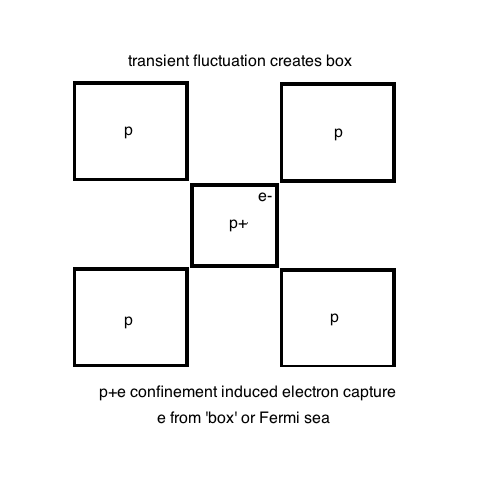
\includegraphics[scale=0.5]{img/box-before.png}
   \caption{Confinement Induced Electron Capture: before}
  \label{fig:box1}
\end{figure}

We write this as

$$E_{box}+p^{+}+e^{-}\rightarrow n^{0}+\nu_{e}$$

where $E_{box}$ represents a \emph{confinement energy}, which is induced by the box constraints. 

After the electron capture event, the box contains a cold neutron, with a very little kinetic energy and a very small mean free path.  Also, as depicted in Figure \ref{fig:box2}, the box now wants to expand because the 'walls', which are effectively a Fermi sea of electrons, are repelling each other and the stabilizing positive charge is gone.

\begin{figure}
   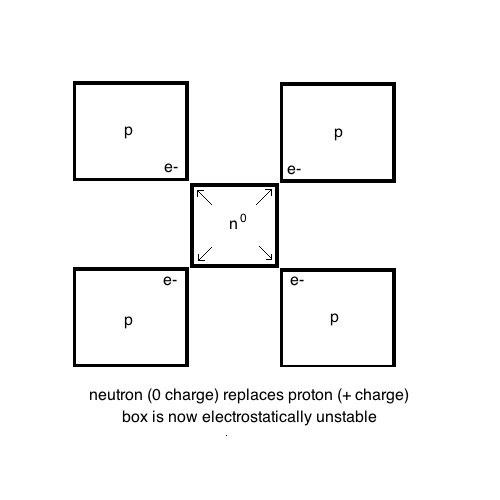
\includegraphics[scale=0.5]{img/box-after.png}
   \caption{Confinement Induced Electron Capture: after}
  \label{fig:box2}
\end{figure}

At this point, shown in Figure \ref{fig:box3}, we imagine the box has effectively expanded, and the neutron can capture a nearby proton, forming deuterium, and releasing of 2.2MeV of energy:  

$$n^{0}+p^{+}\rightarrow d^{+}+2.2MeV$$

\begin{figure}
   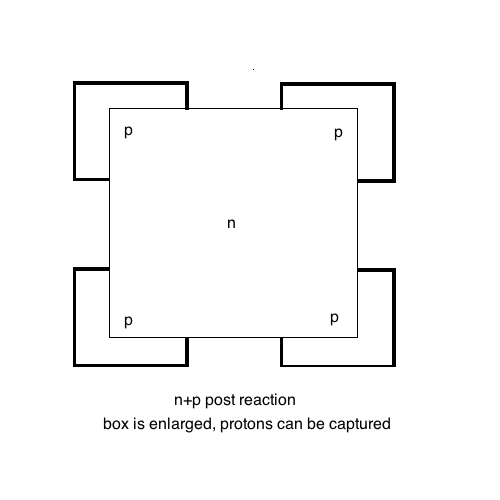
\includegraphics[scale=0.5]{img/box-enlarged.png}
   \caption{Confinement Induced Electron Capture: after}
  \label{fig:box3}
\end{figure}

We would like to understand if such a process is reasonably possible and how to model both the rate of electron capture and the maximum excess power such a process might produce.

Here, we examine what do detailed calculations look like that employ the full machinery of the Weak Interaction, as an illustrative exercise.

Before we describe the theoretical approach, we address a few conceptual issues in setting up the problem.

\subsubsection{Compton length}
The first obvious question is, should we use a classical or a relativisitic box?   

Most electron capture rate calculations use \emph{ab initio} classical wavefunctions,\cite{ec-review1,ec-review2} perhaps with some relativisitic corrections to the electronic Hamiltonian. \cite{martin}

We argue that we can safely use a classical box as long as $L_{min} \ge \frac{1}{2\pi}\lambda_{e}$, where $\lambda_{e}$ is Compton wavelength of an electron. \cite{relbox,compton,planck}  The Compton wavelength sets the scale, accounting for both quantum mechanics and special relativity.

$$\lambda_{e}=\dfrac{h}{m_{e}c}=\dfrac{e^{2}}{m_{e}c^{2}}$$

$$\lambda_{e}\approx2.426\times 10^{-12}\;m$$

For an electron, the minimum L is on the order of 0.004 Angstrom 
$$L_{min}\sim0.004\;\mathring{A}$$ 

In any high energy, relativisitic system, positrons can be produced; here it is through $\beta^{+}$-decay. This generally occurs at or below the Compton length. We are seeking the maximum box size which can induce electron capture, and we assume that, at the maximum, positron emission will be very rare.


If the box is extremely small, and the energy of the electron is of the order of a W boson, we are no longer in the low momentum limit and one would need to consider higher order corrections to the Weak interaction.\cite{klein1}

We also assume that the electron wavefunction does not change appreciably during the interaction, so that we may use a very simplified form for the cross section ($\sigma$) and rate ($\Gamma$).  Again, this is reasonable for boxes $L\ge\lambda_{e}$.


\subsubsection{Confined Atomic systems}

Usually electron capture is described using the atomic orbitals of the parent and daughter nuclei.\cite{ec-review1,ec-review2}  This is very complicated and the basic physical insight can be lost in the details of various angular momentum selection rules and orbital overlap calculations.  Moreover, when an H atom is confined, the electron will detach from the proton and behave like a free particle in a box.\cite{Sen}  


\subsubsection{Pair Production}

We do recognize, however, that in typical cage or other confined environment, there would be an significant thermal effects that may induce positron emission.Indeed, the electron energy needs to be very fine-tuned in order to allow capture but not pair creation.  In the box with multiple electrons, any fine-tuning would be overcome by electron-electron collisions, which would induce energy fluctuations that could drive  pair production.  For example, at high density, assuming a thermal distribution, if there are 800 keV electrons, there would be some 1 MeV electrons, which are enough to cause significant pair creation, probably faster than electron capture.  

Here, we assume that the confinement is a highly transient, far-from-equilibrium process, and that we can ignore pair production from both thermal noise and electron-electron scattering. 

\subsubsection{Klein Paradox}

Klein noted that a relativistic (Dirac) particle-in-a-box will \emph{leak out} at box sizes near, \emph{or above}, the Compton wavelength--this called the Klein paradox. \cite{klein1,klein2}  And while this is usually taught as being simply particle-antiparticle creation, it has been suggested that the Klein paradox it can occur even at larger boxes sizes, and it is a general phenomena of confined relativistic particles.  Recent experiments on Graphene have reopened the debate \cite{klein3}. Still, we will assume the traditional interpretation and we will ignore the Klein paradox.

So we use a classical box, with minimum size $L_{min}=0.004\;\mathring{A}$.  We compute the maximum size below.

\subsubsection{Neutron post-reaction}

To prevent the reverse reaction, we assume that, in the expanded box, the free neutron subsequently combines with another proton, and gives us 2.2 MeV of energy in the process.  This post-process contributes to the power output.  Realistically, we expect this to happen at the maximum box size, at the energy threshold, where the outbound neutron has very low momentum and therefore a very small mean free path.  

Still, for illustrative purposes, we will compute the power output,  assuming this post-reaction,  at all box sizes.

\section{Theory and Calculations}

The electron capture rate can be computed using the Fermi VA theory, \cite{ec-review1,ec-review2}.

\subsection{Particle production under the Weak Interaction}

\begin{figure}
   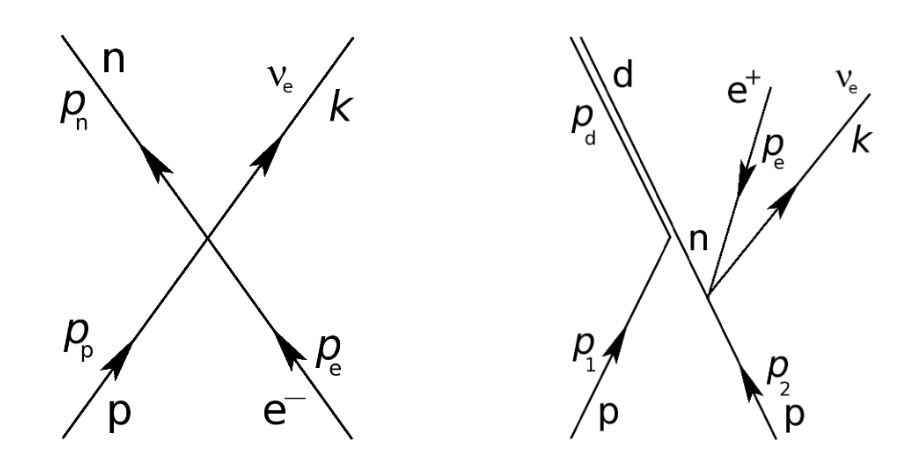
\includegraphics[scale=0.25]{img/feynman.png}
   \caption{EC particle production process}
  \label{fig:ppp}
\end{figure}

Electron capture is mediated by the Weak Interaction, through the particle production process, given by the 4-point Interaction (see Figure \ref{fig:ppp}).   It requires \emph{at least} 0.782 KeV energy to overcome the reaction barrier, which, here, is \emph{provided} by the box. 

$$0.782{KeV}+p^{+}+e^{-}\rightarrow n^{0}+\nu_{e}$$  

We want to compute the rate of E.C. and the (minimum) power generated, as a function of the box size (L), using the full Weak Interaction Hamiltonian.   We will compute the electronic density classically, using box wavefunctions, and, for each box size, determine the incident velocity (as the momentum). We then compute the cross section using the full relativistic kinematics and Dirac spinors.  

To do this, we need to express the rate in terms of the relativistic differential cross section, and in a form suitable for numerical calculations.  
But first, we want to motivate why we use such a complicated form of the cross section.

\subsection{Electron Capture Rates}

Orbital electron capture and other Beta decay processes follow first order kinetics, so the capture rate is described by a single number. 
To calculate the rate, we require a full relativistic, quantum mechanical treatment because the capture process involves both creating particles and the kinetic energy spectrum is of order $m_{e}c^{2}$.

The VA theory is based on second order perturbation theory.  It assumes an incoherent nuclear process, it is local, and that the interaction is phenomenological. It is treated as a simply a contact potential at the surface of the nucleus. Here, this means we need to compute the nuclear charge--the electron density at the the nucleus $\Vert\psi_{e}(R=0)\Vert$, which we obtain from a classical particle-in-the-box wavefunction.

The orbital electron capture rate $\Gamma_{EC}$  is given by multiplying the cross section $\sigma_{EC}$ by the incident velocity $\mathbf{v}^{in}_{ep}$ and (orbital) electron density $\big\vert\Psi_{e}(0)\big\vert^{2}$  at the origin

$$\Gamma_{EC}=\big\vert\Psi_{e}(0)\big\vert^{2}\mathbf{v}^{in}_{ep}\sigma_{EC}\;\;.$$

Of course, this velocity is not relativistic \cite{Cannoni}.  And that is fine for typical calculations.

For example, for something like  $^7Be$ confined in a cage, we assume that $\mathbf{v}^{in}_{ep}$ and $\sigma_{EC}$ are not changing much, and we can estimate the 'cage' rate by n computing the ratio of the confined to uncaged classical molecular electronic densities. 

$$\Gamma^{cage}_{EC}\sim\dfrac{\vert\Psi^{cage}_{e}(0)\vert^{2}}{\vert\Psi^{free}_{e}(0)\vert^{2}}\Gamma^{free}_{EC}$$

And in many other cases, we can just estimate the cross section within a order of magnitude, without worrying about the kinematics.

\subsection{Relativistic Cross Sections}

In our Gedankenexperiment, however, we imagine that the box induces capture, we are at least in the regime of relativistic kinematics.  To that end,
we use a semi-classical, numerical method to describe the electron-capture cross section and perform the rate calculations.
 and using the Lorentz Invariant (LI) scattering cross section for a relativistic ($1+2\rightarrow 3+4$) reaction.  The most basic calculations require a only specifying the electronic wavefunctions(s), averaging over the possible electron-proton momenta, and numerically integrating over the outbound neutrino momentum.    

We could also describe the proton-neutron capture this way, but, for simplicity, we will simply assume the cross section for the post reaction is maximally large, and we ignore the kinematics.  We provide the equivalent expression for the proton-neutron capture cross section in the appendix.

More complicated calculations are used for larger nuclei, second order processes, etc.  They only require modifications to treat either atomic electronic structure of reactant and product atoms, and/or specific considerations for nuclear internal conversion and other second order processes.

We write the Lorentz Invariant (LI) differential cross section in the C.M. frame as

\begin{multline}
d\sigma_{EC}=
\\\left(\dfrac{1}{2\pi}\right)^{2}\dfrac{\sum_{fi}\big\vert\mathcal{M}_{fi}\big\vert^{2}}{16\;\big\vert\mathbf{k}\cdot(E{_n}\mathbf{k}-k^{0}\mathbf{p}_{n})\big\vert}\dfrac{k^{3}p_{e}d\Omega_{k}}{\big\vert\mathbf{p}_{e}\cdot(E_{p}\mathbf{p}_{e}-E_{e}\mathbf{p}_{e})\big\vert}
\end{multline}


where $\mathcal{M}_{fi}$ is a matrix element of the Weak Interaction Hamiltonian,  $\mathbf{k}$ represents the neutrino momentum components $(k^{0},\mathbf{k})=(E_{\nu},\mathbf{k})=p^{4}_{\nu}$,  and we use natural units $(\hbar=1,c=1)$.

This can be readily derived from the standard LI differential cross section for a relativistic ($1+2\rightarrow 3+4$) elastic scattering reaction in the C.M. frame.  It is not commonly used in the literature and it is this form that  allows us to perform detailed numerical rate calculations.

\subsubsection{Rate}

This gives the (differential) rate as

\begin{multline}
d\Gamma_{EC}=\\
\left(\dfrac{1}{2\pi}\right)^{2}\dfrac{\sum_{fi}\big\vert\mathcal{M}_{fi}\left[p_{ep}\rightarrow i\nabla)\right]\psi_{ep}(\mathbf{x})\big\vert_{\mathbf{x}=0}\big\vert^{2}}{16E_{p}E_{e}\;\big\vert\mathbf{k}\cdot(E{_n}\mathbf{k}-k^{0}\mathbf{p}_{n})\big\vert}k^{3}d\Omega_{k}
\end{multline}

where we explicitly specify the electronic wavefunction.

We represent the $(e^{-},p^{+})$ pair using a 3D box wavefunction, and obtain the Energies and 3-momenta from the relativistic kinematics.  

As usual, we average over the initial spins, and sum over the final spins.  That is, we average over all 8 permutations of the incident velocities (really momenta $\mathbf{p}_{ep}$) for the 3D box, and integrate over outbound neutrino solid angle $d\Omega_{k}$ using numerical quadrature.  The final rate is computed as, for each box size, as a function the kinematics, using

$$\Gamma_{EC}=\frac{re1}{8}\sum_{\mathbf{p}_{pe}}\int_{d\Omega_{k}}d\Gamma_{EC}$$

where $\big\vert\mathbf{p}_{ep}\big\vert$ is given by the box size (described below).

\subsubsection{Power}

We  estimate the excess power generated by the confined electron capture, resulting if/when the outbound neutron reacts with the environment. 
The power $\mathcal{P}$ is

$$\mathcal{P}=\Gamma_{EC}*Q*\rho$$

where is the nuclear decay energy, or Q-value, and $\rho$ is the  density of confined elements.  

We don't actually know $\rho$, and as a placeholder we can choose the density to that of a typical material, of order Avogadro's number, $\mathrm{N_{A}}\sim6.02\times10^{23}$.  We will be examining power ratios, so this choice is irrelevant.

We estimate the power for both the bare proton-electron capture

$$\mathcal{P}_{pe}=\Gamma_{EC}*\left[(\mathbf{E}_{e}-m_{e})+(\mathbf{E}_{p}-M_{p})\right]*\rho$$

and the subsequent neutron post-reaction

$$\mathcal{P}_{n}=\Gamma_{EC}*\left[2.2+(\mathbf{E}_{n}-M_{n})\right]*\rho$$.

assuming that the post-reaction has a 

We also define an excess maximum power as

$$\mathcal{P}_{XS}=\mathcal{P}_{pe}-\mathcal{P}_{n}$$

which we argue is a good measure of the gross maximum potential reactive power output of the confined E.C. process. 

Of course, if the outbound neutron has any considerable velocity $v_{n}$, the proton-neutron cross-section $\sigma_{p+n}$ would be very small.  It proton-neutron cross section scales inversely with the velocity ($\sigma_{p+n}\sim\frac{1}{v_{n}}$).  In principle, we could also compute this cross section using the Weak Interaction and the relativistic kinematics, as we did for electron capture.  

But we are only interested in box lengths where the excess power is significant enough to drive the reaction, where the outbound neutron is moving very slow, or is \emph{ulta cold}.  This is, of course, when the box is very large.

\subsubsection{Particle-in-the-box Wavefunctions}

While most electron capture calculations assume a specific, bound, atomic electronic wavefunction(s), we perform a much simpler calculation; we treat the electron-proton pair as classical particle-in-a-box,  and analyze the problem just above the Compton scale using the low order VA theory.  Write the wavefunction as

$$\psi_{ep}(\mathbf{x})=\left(\dfrac{2}{L}\right)^{\frac{3}{2}}cos\left(\dfrac{\pi x}{L}\right)cos\left(\dfrac{\pi y}{L}\right)cos\left(\dfrac{\pi z}{L}\right)$$.

Because the VA theory assumes an incoherent process, the electron, proton wavefunction is usually factored as an electron wavefunction, with a point-particle in the center

$$\psi_{ep}(\mathbf{x})=\psi_{p}(0)\psi_{e}(\mathbf{x})$$

We only consider the ground state $\psi_{ep}^{0}$ wavefunction.

We note, in \emph{ab initio} electronic structure calculations, it is now generally possible to treat the Hydrogen proton wavefunction explicitly, and to treat the electron-proton coupling at the level of Hartree Fock \cite{martin}.  This has proved useful, for example, for describing isotope effects on electronic structure.  It is may also be possible to eventually treat this problem using fully relativistic \emph{ab initio} QFT methods, although this has only been applied to positronium so far \cite{positroniumQFT}.

Here, we treat the confined electron, proton pair in the C.M. frame so that the 3-momentum of the electron and proton are related as
$$\mathbf{p}_{e}=\mathbf{p}_{pe}$$
$$\mathbf{p}_{p}=-\mathbf{p}_{pe}$$

and we consider all 8 permutations for each given box size L:

$$\pm\mathbf{p}_{pe}(1), \pm\mathbf{p}_{pe}(1), \pm\mathbf{p}_{pe}(3)$$

\subsubsection{Relativistic Kinematics and Energetics}
For consistency with the particle production process, we treat all kinematics and energetics relativistically.  Given energy-momentum conservation

$$E^{2}=m^{2}+\mathbf{p}^{2}$$

and the 3D particle-in-the-box energy ground state energy 

$$E_{gs}=\dfrac{3\pi^{2}}{2mL^{2}}\;\;,$$

we use $E=\dfrac{\mathbf{p}^{2}}{2m}$ to write

$$E^{2}_{e}=m^{2}_{e}+3\left(\dfrac{\pi}{L}\right)^{2}\;\;,$$ and

$$E^{2}_{p}=M^{2}_{p}+3\left(\dfrac{\pi}{L}\right)^{2}\;\;.$$

The threshold Kinetic energy in the center of momentum (C.M.) frame is given as

$$EKe_{min}:\;\;K_{e}=E_{e}-m_{e}=\dfrac{(M_{n}-m_{e}+m_{\nu})^{2}-M^{2}_{p}}{2(M_{n}+m_{\nu})}$$

which is approximately 781.6 KeV (or 783.1 KeV in the proton rest frame).

Of course, the proton rest frame is approximately the electron rest frame, but it should be mentioned that the in the electron rest frame, the threshold kinetic energy is 2000X greater.  Therefore, it is assumed that the energy transfer to induce electron capture is in the C.M. frame of the (e,p) pair.

The minimum momentum is 

$$\mathbf{p}_{min}=\sqrt{(K_{e}+m_{e})^{2}-m_{e}^{2}}\;\;.$$

For the final state, the neutrino $(\nu)$ kinetic energy is

$$K_{\nu}=k^{0}-m_{\nu}=\dfrac{(E_{p}+E_{e}-m_{\nu})^{2}-M^{2}_{n}}{2(E_{p}+E_{e})}$$

and the neutron $(n)$ kinetic energy is

$$K_{n}=E_{n}-M_{n}=\dfrac{(E_{p}+E_{e}-M_{n})^{2}-m^{2}_{\nu}}{2(E_{p}+E_{e})}$$

At this point, we can compute the relativistic energies for all particles, simply as a function of box length (L), for a confined $(e^{-},p^{+})$ pair.  Of interest is the shape of the curve, and when the excess power output becomes favorable.  

To compute the exact rate and estimate the power, we need to evaluate the matrix element(s) of the Weak Interaction Hamiltonian.  
While most practitioners simply estimate this, for our purpose, we can simply compute them exactly.

\subsection{Weak Interaction Hamiltonian and Matrix Elements}

The Hamiltonian for the VA theory for E.C. is \cite{ec-review1,ec-review2,langanke} 

$$\mathcal{H}(x)=-\dfrac{G_{F}}{\sqrt{2}}\left[J^{\mu}(x)L^{+}_{\mu}(x)+h.c.\right]$$

where $J^{\mu}$ and $L_{\mu}$ are (in modern parlance) the Hadron and Lepton currents, resp., and are given by

$$J_{\mu}=\bar{u}_{n}\gamma_{\mu}(1+\lambda\gamma_{5})u_{p}$$

$$L_{\mu}=\bar{u}_{\nu}(1-\gamma_{5})u_{e}$$

where $u_{n},u_{p},u_{e},u_{\nu}$ are Dirac (free-particle) wavefunctions.   

Notice that we are only interested in semi-leptonic processes, governed by weak changing currents, and only leptons are electrons.  

$G_{F}$ is the Universal Fermi Weak Coupling Constant, and $\lambda=-\dfrac{G_{A}}{G_{V}}$, which is determined by experiment (and subject to minor changes). 
 $G_{V}$ is the Axial-Vector Weak Coupling Constant, and $G_{A}$ is the vector weak coupling
constant.  The most recent value is $G_{V}=1.2767(16)$, and $G_{A}=1$ \cite{vacoupling}.

\subsubsection{VA Matrix Elements}

In our calculations, however, we use a slightly different, more modern convention for the matrix elements, multiplying through by $G_{V}$ \cite{zuber}.   The matrix elements $\mathcal{M}_{fi}$ are then given by

\begin{multline}
\mathcal{M}_{fi}=\dfrac{G_{F}}{\sqrt{2}}\bar{u}(p_{n},s_{n})(G_{V}-G_{A}\gamma^{5})\gamma^{\mu}u(p_{p},s_{p})\times \\
\bar{u}(p_{\nu},s_{\nu})\gamma_{u}(1-\gamma^{5})u(p_{e},s_{e})
\end{multline}

where $u{(p},s)$ are Dirac 4-spinors, with the convention 

$$u{(p},s=1)=\sqrt{E+m}\left[\begin{array}{c}
1\\
0\\
\frac{p_{3}}{E+m}\\
\frac{p_{1}+ip_{2}}{E+m}
\end{array}\right]$$
$$u{(p},s=2)=\sqrt{E+m}\left[\begin{array}{c}
0\\
1\\
\frac{p_{1}-ip_{2}}{E+m}\\
\frac{p_{3}}{E+m}
\end{array}\right]$$

$$\langle\bar{u}|u\rangle=\bar{u}_{0}u_{0}-\bar{u}_{1}u_{1}-\bar{u}_{2}u_{2}-\bar{u}_{3}u_{3}$$

and $\bar{u}=u^{\dagger}\gamma^{0}$.  The $\gamma$ are 4-component Gamma matrices, and  $(\cdots\gamma^{\mu}\cdots\gamma_{u}\cdots)$ is the Einstein summation convention. 

Recall that the VA theory assumes that the electron-proton interaction is a contact potential, operating at the surface of the nucleus, and that the underlying quantum process is incoherent.    We need simply compute the matrix elements in terms of the terms of the individual Hadronic and Leptonic currents

$$\mathbf{J}_{had}=\bar{u}(p_{n},s_{n})(G_{V}-G_{A}\gamma^{5})\gamma^{\mu}u(p_{p},s_{p})$$

$$\mathbf{L}_{lep}=\bar{u}(p_{\nu},s_{\nu})\gamma_{u}(1-\gamma^{5})u(p_{e},s_{e})$$.

\subsubsection{Sum over spin combinations}

Electron capture is similar to Beta decay in that there are allowed (Singlet-like) and disallowed (Triplet-like) transitions,
as well as some very low order disallowed contributions.  These are, of course, different from Beta decay since we need to consider the total angular momentum of the initial ($p^{+}+e^{-
})$ and final $(n^{0}+\bar{\nu_{e}})$ states.  

Typically we identify Fermi and Gamow-Teller states in terms of total isospin, meaning $s_{n}=s_{\nu}$ or $s_{n}\neq s_{\nu}$. 
 
Here, by Singlet-like states, we  mean total spin 0, and by Triplet-like, we mean total  spin $1$ or $-1$.  Here we find that states of total spin 0 (hadronic and leptonic) have the same order of magnitude.   Since we are using particle-in-the-box electronic wave functions,  we do not consider orbital angular momentum, and therefore only have to consider if $s_{p}=s_{e}$ or  $s_{n}=s_{\nu}$. Notice, however, we use the Dirac-spinor convention for $s=1\;(up)$ and $s=2\;(down)$, so total $s=0$ corresponds to ($up,down$) or ($down,up$), etc.

\begin{figure}
   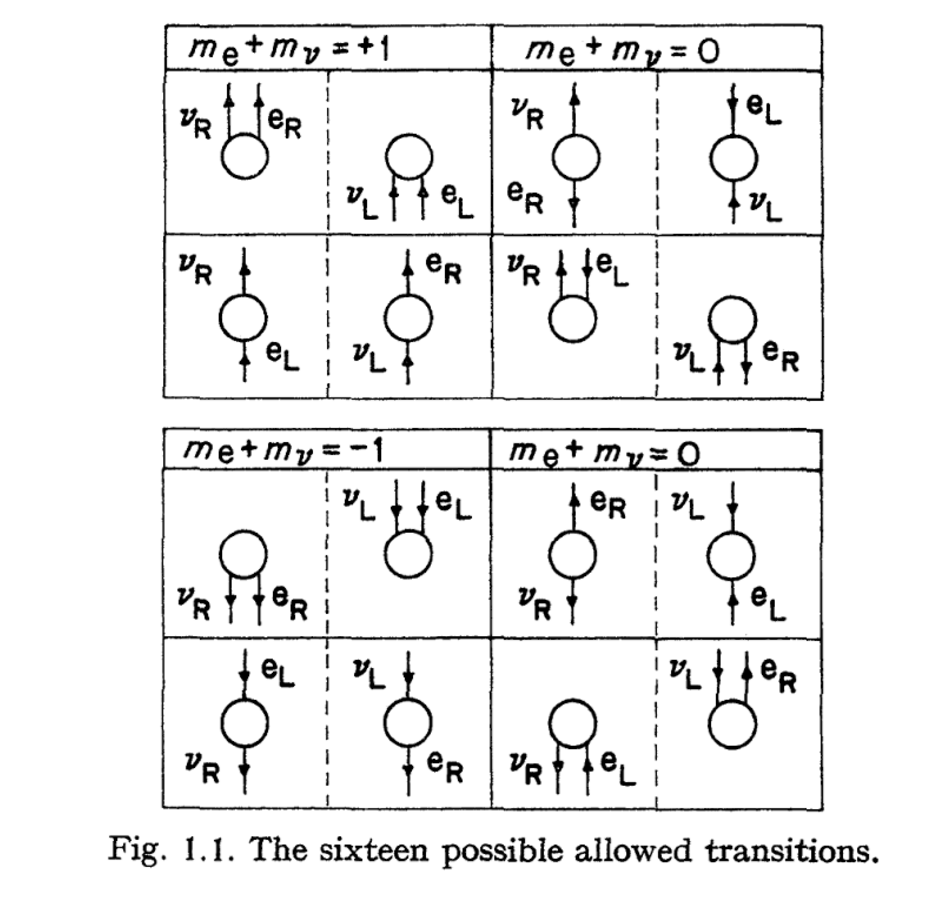
\includegraphics[scale=0.5]{img/16-allowed.png}
   \caption{Allowed spin transitions}
  \label{fig:SC}
\end{figure}
We sum over the 16  allowed transitions in the VA theory, as depicted in Figure \cite{fig:SC}
 (taken from Beta decay for Pedestrians; we need to replicate , but use p-e as the states, not e-k)

We observe four dominant (\emph{allowed}) spin combinations, 
consisting of Singlet-like initial and final states,  which is of order $50$ (in natural units)

$$s_{p}\neq s{_e};\;\;\;s_{n}\neq s_{\nu}$$
$$\bar{u}(p_{n},1)u(p_{p},1)\;\bar{u}(p_{\nu},2)u(p_{e},2)$$
$$\bar{u}(p_{n},2)u(p_{p},2)\;\bar{u}(p_{\nu},1)u(p_{e},1)$$,
$$\bar{u}(p_{n},2)u(p_{p},1)\;\bar{u}(p_{\nu},1)u(p_{e},2)$$
$$\bar{u}(p_{n},1)u(p_{p},2)\;\bar{u}(p_{\nu},2)u(p_{e},1)$$.

There are two weaker (\emph{dis-allowed}) combinations, 
where are all spins are the same (Triplet-like states), and are of order $10^{-1}$ (that is, $10^{-3}$ smaller in magnitude)

$$s_{n}=s_{p}=s_{\nu}=s{_e}$$
$$\bar{u}(p_{n},1)u(p_{p},1)\;\bar{u}(p_{\nu},1)u(p_{e},1)$$
$$\bar{u}(p_{n},2)u(p_{p},2)\;\bar{u}(p_{\nu},2)u(p_{e},2)$$.

There are four remaining, non-zero contributions, consisting of a single spin flip
in the initial or final state, and is of order $10^{-3}$ in magnitude

$$s_{p}\neq s{_e}\;{or}\;s_{n}\neq s_{\nu}$$

$$\bar{u}(p_{n},1)u(p_{p},1)\;\bar{u}(p_{\nu},1)u(p_{e},2)$$
$$\bar{u}(p_{n},2)u(p_{p},2)\;\bar{u}(p_{\nu},2)u(p_{e},1)$$.
$$\bar{u}(p_{n},2)u(p_{p},1)\;\bar{u}(p_{\nu},2)u(p_{e},2)$$
$$\bar{u}(p_{n},1)u(p_{p},2)\;\bar{u}(p_{\nu},1)u(p_{e},1)$$


The remaining (single and double flip) transitions have zero amplitude.

\subsection{Numerical Calculations}

We outline the calculations in pseudocode below.  

The full calculations sums of over all 8 possible incident momenta permutations
  $(\pm\mathbf{p}_{ep}(1),\pm\mathbf{p}_{ep}(2),\pm\mathbf{p}_{ep}(3) )$,
and the 16 allowed spin transitions (see figure below). By conservation of momenta, we can eliminate the neutron and only need to average over the outbound neutrino momenta solid angle ($d\Omega_k$); we do this using an 8-point gaussian quadrature. 


 \begin{figure*}
 \begin{minipage}{\linewidth}
\begin{algorithm}[H]
\caption{Rate and Power Calculations}\label{code}
\begin{algorithmic}[1]
\For{$\mathsf{p}_{ep}\in [\mathsf{p}_{max}, \mathsf{p}_{min}]$}\Comment{$\mathsf{p}_{ep}=\|\mathbf{p}_{ep}(L)\|$}
\State $Tran(\mathsf{p}_{ep})=0$\Comment{Transfer}
\State $Power_{n}(\mathsf{p}_{ep})=0$\Comment{Neutron Power}
\For{$w_{x},w_{\phi}\in \mathbb{Q}[1,8]$}\Comment{quadrature weights}
\For{$s_{n},s_{p},s_{\nu},s_{e}\in [0, 1]$}\Comment{$s_{up},s_{down}=0,1$}
\For{$s_{x},s_{y},s_{z}\in [-1,1]$}\Comment{$\mathbf{p}_{ep}=\mathsf{p}_{ep}[s_{x},s_{y},s_{z}]$}
\State $p_{n},p_{p}, p_{\nu},p_{e}, \gets pekin(w_{x},w_{\phi},\mathbf{p}_{ep})$\Comment{4 vectors $\gets$ rel. kinematics}
\State $\bar{u}(p_{n},s_{n}),u(p_{p},s_{p}), \bar{u}(p_{\nu},s_{\nu}), u(p_{e},s_{e})$\Comment{spinors by p, s-index}
\For{$u\in[1,4]$}\Comment{4-vector indices}
\State $\mathbf{J}_{had}=\bar{u}(p_{n},s_{n})\cdot(G_{V}-G_{A}\gamma^{5})\cdot\gamma^{\mu}\cdot u(p_{p},s_{p})$\Comment{Hadronic current}
\State $\mathbf{L}_{lep}=\bar{u}(p_{\nu},s_{\nu})\cdot\gamma_{u}\cdot(1-\gamma^{5})\cdot u(p_{e},s_{e})$\Comment{Leptonic current}
\EndFor
\State $\mathbb{C}=\langle\mathbf{L}^{\dagger}_{lep},\mathbf{J}_{had}\rangle$\Comment{Current Amplitude}
\EndFor
\EndFor
\State $\mathcal{F}^{2}(\mathsf{p}_{ep},p_{p},p_{e}, p_{n}, p_{\nu})$\Comment{Matrix Element Factor}
\State $Tran(\mathsf{p}_{ep})+=w_{x}w_{\phi}Re[\mathbb{C}^{\dagger}\mathbb{C}]\mathcal{F}^{2}$\Comment{Integrated Rate}
\EndFor
\State $P_{n}(\mathsf{p}_{ep})=Tran(\mathsf{p}_{ep})*(2.2+(E_{n}-M_{n}))$\Comment{Neutron Power estimate}
\EndFor
\end{algorithmic}
\end{algorithm}
\end{minipage}
\end{figure*}


Let us write the Real part of the current density as

$$C^{2}_{Re}=Re(\bar{C}^{2}_{amp}{C}^{2}_{amp})$$

where

\begin{multline}
C^{2}_{amp}=(\mathbf{J}_{had})^{\mu}(\mathbf{L}_{lep})_{\mu}=\\
J^{0}_{had}L^{0}_{lep}-J^{1}_{had}C^{1}_{lep}-J^{2}_{had}L^{2}_{lep}-J^{3}_{had}L^{3}_{lep}
\end{multline}

We  express the rate as

$$\Gamma_{EC} = C^{2}_{Re}(\mathcal{F})$$

in terms of an intermediate factor
\begin{multline}
\mathcal{F}=r_{c}\left(\dfrac{p_{ep}}{2\pi}\right)^{3}\left(\dfrac{G_{F}^{2}(E_{\nu}^{2}-m_{\nu}^{2})^{3}}{512\pi^{2}\;E_{p}E_{e}\hbar c\;\big\vert\; \mathbf{k}(E_{n}p_{\nu}-E_{\nu}p_{n})\;\big\vert}\right)
\end{multline}

We write the two power terms as
$$P1 = P_{pe}=C^{2}_{Re}\left[(\mathbf{E}_{e}-m_{e})+(\mathbf{E}_{p}-M_{p})\right]\left(\mathcal{F}\right)$$
$$P2 =P_{n}=C^{2}_{Re}\left[2.2+(\mathbf{E}_{n}-M_{n})\right]\left(\mathcal{F}\right)$$

and compute these as a function of the box size using the relativistic kinematic and Weak Interaction matrix elements.  We are interested in the estimated neutron output power ratio 

$$power\;ratio:\;\dfrac{P_{n}}{P_{ep}}$$

as a function of box length $L$.

\subsection{Results}

\begin{figure*}
 \begin{minipage}{\linewidth}
   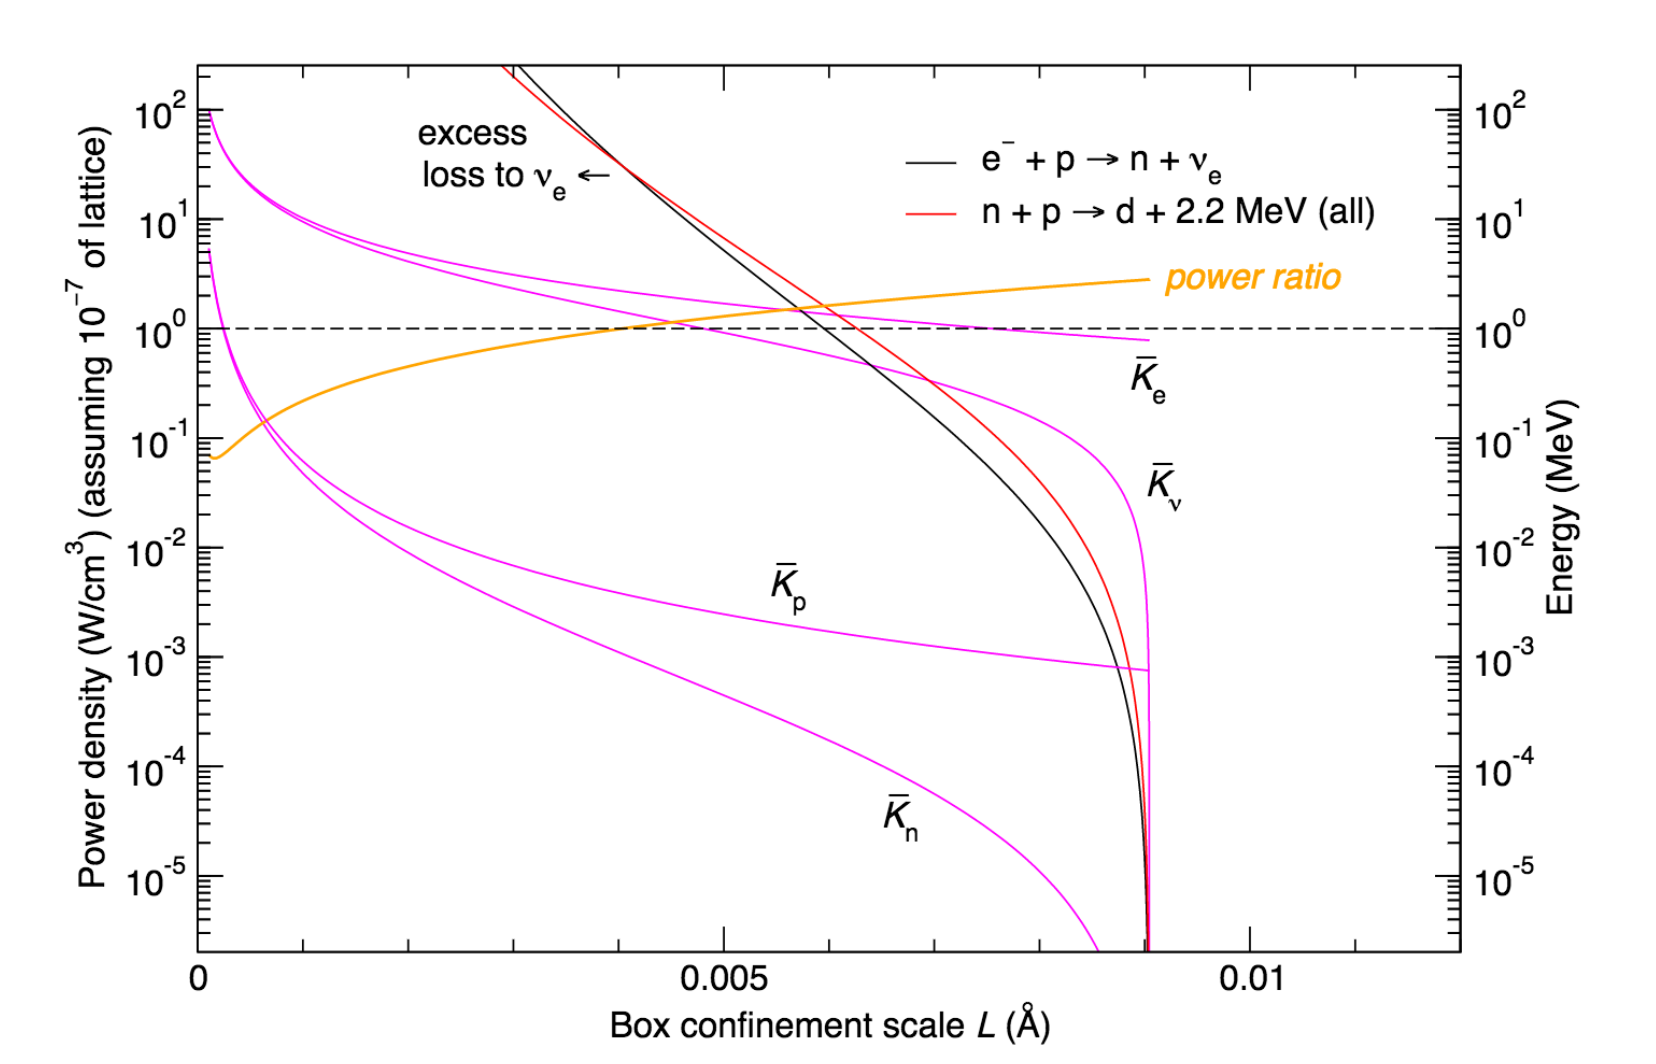
\includegraphics[scale=0.5]{img/results.png}
   \caption{Kinetic Energy and Power as a function of Box Length}
  \label{fig:results}
\end{minipage}
\end{figure*}


Figure \ref{fig:results} presents the results of relativistic kinematics and excess power calculations, as a function of box length.
For illustrative purposes, we include results box sizes even below the Compton length.  The excess power ratio is greater than unity for $L>0.004\mathring{A}$, with a maximum of almost a factor of 3.


These simple calculations indicate that a confined electron capture reaction would be favorable as long as the produced neutrons react with environment at a high rate.  This is expected at the maximum box size, where the neutron has the smallest mean free path, although the reaction appears favorable for all box lengths larger than the Compton length,$L>0.004\mathring{A}$.

\section{Discussion}

We present calculations for a Gedankenexperiment describing confined orbital electron capture of a bare proton and an electron in a box

$$E_{box}+p^{+}+e^{-}\rightarrow n^{0}+\nu_{e}$$

 The intent is to model, conceptually, a confined proton, trapped in a field of free electrons, such that the kinetic energy of the proton is high enough to induce electron capture.  We treat system as an electon-proton pair in a classical particle-in-the-box, and compute the capture rate using the Fermi VA theory.  We use classical box wavefunctions to express the confinement, and compute relativistic proton momentum and kinetic energy resulting from the box.  We then compute the  rate by evaluating the Weak Interaction Hamiltonian matrix elements using the box wavefunction density at the origin, using a form of the Lorentz Invariant differential cross section that takes into account the full relativistic Kinematics of  $(1+2\rightarrow 3+4)$ elastic scattering nuclear reactions.  We  compute the power generated by the E.C. process, as well as estimate the minimum excess neutron power, as a function of box size $L$.  We find that the excess power ratio is greater than one for box sizes $L>0.004\mathring{A}$, and increases rapidly as we approach the maximum box size $L>0.009\mathring{A}$.  We note we need a compression ratio of order 50X to induce capture.

While being pedagogic exercise, we would also like to discuss both directions for future work and a possible application.

\subsection{Low energy electron-proton scattering resonances}
We treat the electron-proton pair as if they are bound by the box potential; that is, we assume the box exists.
We would like to observe a bound state directly, but describing bound states in relativistic field theory is a complex problem.
Indeed, Steven Weinberg has stated \cite{weinberg}:

\emph{It must be said that the theory of relativistic effects and radiative corrections in bound states is not yet in satisfactory shape.�}

Ideally we would look for resonances, or quasi-bound states, in solutions of the Bethe Salpeter equation, or a related formulation of the relativistic two-body equations, for electron-proton scattering.  This is significantly more complicated, requires some choice of approximation, and is prone to singularities that can lead to numerical instabilities.  Still, there is some older work that suggests this may be successful.  

In 1991, Spence and Vary claimed to have observed several (5) narrow, low energy, near threshold continuum resonances in numerical solutions of the Blankenbeckler-Sugar equation, a specific, relativistic (but not Gauge invariant) reduction of the two-body Bethe-Salpeter equation into a one-body equation. Their results suggested there could be short lived, quasi-bound electron-proton states up to 100 fm ($0.001\mathring{A}$) in extent.  This is of order the box sizes we have investigated, and it would be very interesting to continue out study of confined electron capture using modern techniques.  

The best, modern, relativistic \emph{ab initio} techniques so far, also by Vary, have successfully treated positronium,\cite{positroniumQFT} and it would be interesting to try to extend such methods to electron-proton scattering. This is significantly more difficult since most \emph{ab initio} many body methods can treat ground states, but to find quasi-bound states  requires a powerful open shell method.

\subsection{Confinement-induced Nuclear Fusion in the Earth's Inner Core}

We briefly mention a recent proposal for another type of  confinement-induced nuclear reaction,
namely, nuclear fusion at the Earth's core.

The source of heat from the Earth's crust remains controversial, although heat flow
to the surfaces seemingly arises from both primordial and radiogenic sources.
Moreover, signatures of antineutrinos have been detected emanating from the core.
Recently (2016), Fukuhara proposed that the observed heat and geoneutrinos
result from a three-body nuclear fusion of deuterons.\cite{fukuhara}  They argue that
the reaction occurs in D atoms confined in hexagonal FeDx crystals, at high pressure
and temperature.  Moreover, the D+D+D collision is modulated by a charge density wave
instability which causes a breathing-mode-like displacement of the deuterons.

It is noted that the confinement is estimated to be $37\%$ of equilibrium lattice constant,
of order a Bohr radius ($0.5\mathring{A}$).  This is significantly larger than the L values here,
although fusion requires a significantly smaller level of confinement than electron capture.
And we do not consider temperature or pressure effects in our model, which Fukuhara
estimates includes another $50\%$ confinement in this model.

\begin{acknowledgments}
We wish to acknowledge the support of the Anthropocene Institute for proving funding for this work.

\end{acknowledgments}
%\nocite{*}
\bibliography{EC-aipsamp}% Produces the bibliography via BibTeX.

\end{document}
%
% ****** End of file aipsamp.tex ******
